\subsection{Efficacité surfacique}

Observant le fichier \texttt{cache.cfg}, on constate que la capacité totale des données pouvant être stockées dans le cache, sans compter les métadonnées telles que les \emph{tags}, identifiée comme la taille du cache, est de 131072~bytes, soit 128~KiB. De son côté, l’unité minimale chargée depuis la mémoire ou depuis le niveau \texttt{L2} vers le cache correspond à la taille de bloc, qui est de 64~bytes. La configuration standard comporte 2~voies pour le placement des blocs à l’intérieur des ensembles (\emph{sets}). Enfin, la technologie utilisée par défaut est de 0{,}090~$\mu$m, soit 90~nm.

Les surfaces proviennent des sorties CACTI (\texttt{cacti/result\_L1\_*}) via la ligne
\texttt{Cache height x width (mm)}. 
En supposant les tailles du Tableau~12 : L1I = L1D = 16\,kB (A7) et 32\,kB (A15), on obtient :

\begin{table}[h]
\centering
\footnotesize
\begin{tabular}{lccc}
\hline
\textbf{Cœur} & $S_{L1I}$ (mm$^2$) & $S_{L1D}$ (mm$^2$) & $S_{L1}=S_{L1I}+S_{L1D}$ (mm$^2$) \\
\hline
A7 (16\,kB)  & 0{,}03774 & 0{,}03774 & 0{,}07548 \\
A15 (32\,kB) & 0{,}03319 & 0{,}03319 & 0{,}06639 \\
\hline
\end{tabular}
\end{table}

Avec $S_{\text{core+L1}}(A7)=0{,}45$ mm$^2$ et $S_{\text{core+L1}}(A15)=2$ mm$^2$ :
\[
\%L1(A7)=\frac{0{,}07548}{0{,}45}\times 100 = 16{,}77\%,
\qquad
\%L1(A15)=\frac{0{,}06639}{2}\times 100 = 3{,}32\%.
\]
\[
S_{\text{core hors L1}}(A7)=0{,}45-0{,}07548=0{,}37452~\text{mm}^2,
\quad
S_{\text{core hors L1}}(A15)=2-0{,}06639=1{,}93361~\text{mm}^2.
\]

\textbf{Analyse.} Le A7 consacre une fraction beaucoup plus importante de sa surface au L1
($\approx 16{,}8\%$) que le A15 ($\approx 3{,}3\%$), ce qui reflète un cœur plus compact :
à taille de L1 comparable, le poids surfacique est plus élevé sur A7.

\paragraph{Q8.}
Les surfaces L1 (I et D) sont celles de CACTI (\texttt{cacti/result\_L1\_*}). 
Le L2 fixé à 512\,kB donne, avec les paramètres gem5 (A7: 32\,B, 8-way ; A15: 64\,B, 16-way),
\[
S_{L2}(A7)=0{,}94241~\text{mm}^2, \qquad S_{L2}(A15)=0{,}94019~\text{mm}^2.
\]
Pour chaque taille L1, on utilise :
\[
S_{\text{core+L1+L2}} = S_{\text{core hors L1}} + 2S_{L1} + S_{L2}.
\]

\begin{table}[h]
\centering
\footnotesize
\begin{tabular}{c|ccc}
\hline
\textbf{L1 (kB)} & $S_{L1}$ (mm$^2$) & $S_{L1}^{\text{tot}}$ (mm$^2$) & $S_{\text{core+L1+L2}}$ (mm$^2$) \\
\hline
\multicolumn{4}{c}{\textbf{Cortex-A7 (L2=512\,kB, 32\,B, 8-way)}}\\
1  & --      & --      & -- \\
2  & 0{,}01719 & 0{,}03438 & 1{,}35130 \\
4  & 0{,}02095 & 0{,}04189 & 1{,}35882 \\
8  & 0{,}02652 & 0{,}05304 & 1{,}36996 \\
16 & 0{,}03774 & 0{,}07548 & 1{,}39241 \\
\hline
\multicolumn{4}{c}{\textbf{Cortex-A15 (L2=512\,kB, 64\,B, 16-way)}}\\
2  & 0{,}00433 & 0{,}00867 & 2{,}88247 \\
4  & 0{,}00495 & 0{,}00990 & 2{,}88370 \\
8  & 0{,}01432 & 0{,}02865 & 2{,}90245 \\
16 & 0{,}01767 & 0{,}03534 & 2{,}90914 \\
32 & 0{,}03319 & 0{,}06639 & 2{,}94019 \\
\hline
\end{tabular}
\end{table}

\textit{Note :} CACTI ne trouve pas d’organisation valide pour A7 à 1\,kB (d’où ``--'').

\paragraph{Graphes (pgfplots).}
\begin{figure}[h]
\centering
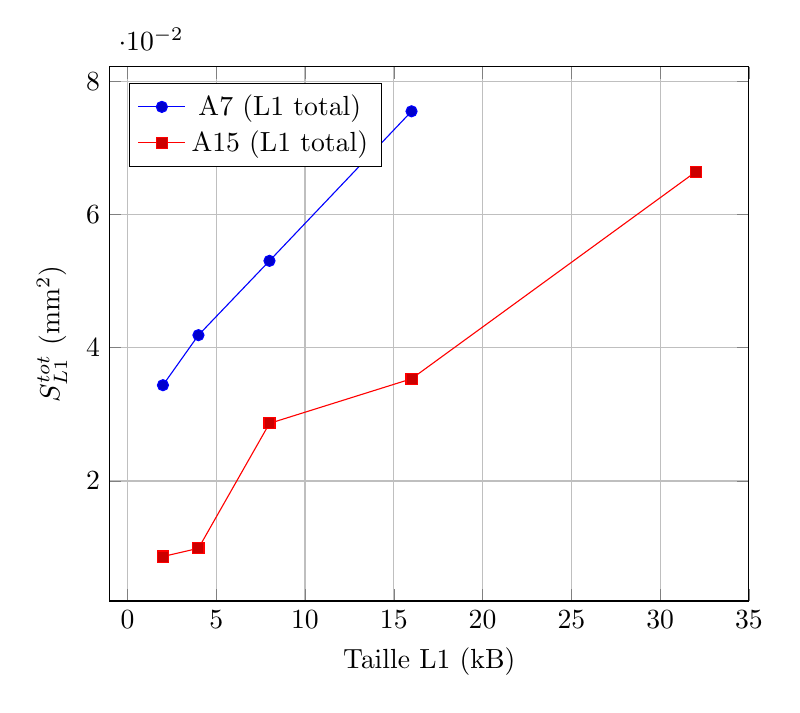
\begin{tikzpicture}
\begin{axis}[
    width=0.8\linewidth,
    xlabel={Taille L1 (kB)},
    ylabel={$S_{L1}^{tot}$ (mm$^2$)},
    legend pos=north west,
    grid=both
]
\addplot coordinates {(2,0.03438) (4,0.04189) (8,0.05304) (16,0.07548)};
\addlegendentry{A7 (L1 total)}
\addplot coordinates {(2,0.00867) (4,0.00990) (8,0.02865) (16,0.03534) (32,0.06639)};
\addlegendentry{A15 (L1 total)}
\end{axis}
\end{tikzpicture}
\caption{Surface totale des L1 (I+D) en fonction de la taille.}
\end{figure}

\begin{figure}[h]
\centering
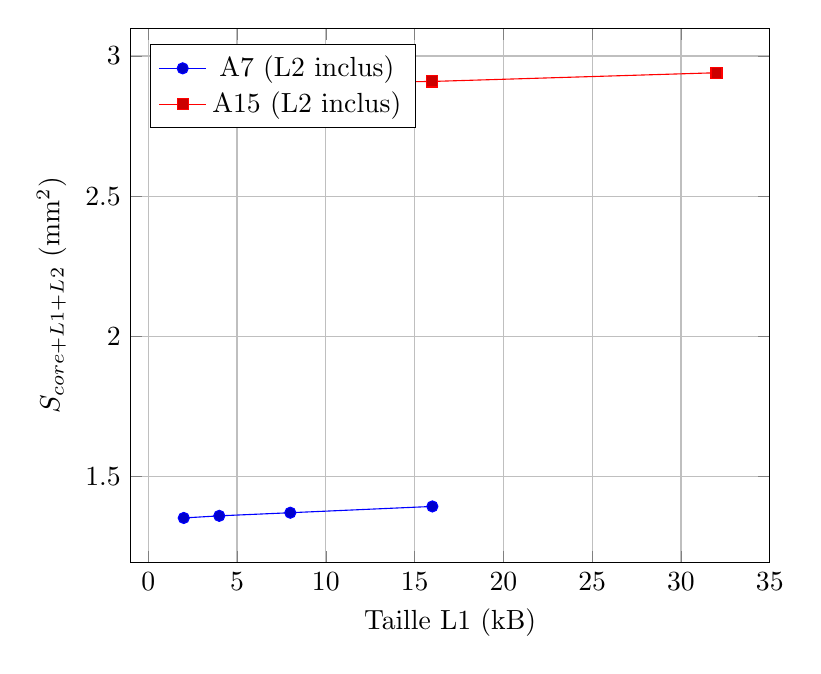
\begin{tikzpicture}
\begin{axis}[
    width=0.8\linewidth,
    xlabel={Taille L1 (kB)},
    ylabel={$S_{\text{core+L1+L2}}$ (mm$^2$)},
    legend pos=north west,
    grid=both
]
\addplot coordinates {(2,1.35130) (4,1.35882) (8,1.36996) (16,1.39241)};
\addlegendentry{A7 (L2 inclus)}
\addplot coordinates {(2,2.88247) (4,2.88370) (8,2.90245) (16,2.90914) (32,2.94019)};
\addlegendentry{A15 (L2 inclus)}
\end{axis}
\end{tikzpicture}
\caption{Surface totale des cœurs (L1 variable + L2=512\,kB).}
\end{figure}


\paragraph{Efficacité surfacique.}
On utilise les IPC issus des fichiers CSV (par processus et par taille de L1) et la surface
totale du cœur avec L2 fixe (512\,kB) :
\[
\eta = \frac{IPC}{S_{\text{total}}}\quad\text{avec}\quad
S_{\text{total}} = S_{\text{core hors L1}} + 2S_{L1} + S_{L2}.
\]
Ici $S_{L2}(A7)=0{,}94241$~mm$^2$ et $S_{L2}(A15)=0{,}94019$~mm$^2$.
Les valeurs suivantes sont donc en $IPC/\text{mm}^2$.

\begin{table}[h]
\centering
\footnotesize
\begin{tabular}{c|cccc}
\hline
\textbf{L1 (kB)} & \textbf{Dijkstra small} & \textbf{Dijkstra large} & \textbf{Blowfish small} & \textbf{Blowfish large} \\
\hline
\multicolumn{5}{c}{\textbf{Cortex-A7}}\\
1  & --      & --      & --      & -- \\
2  & 0,1787  & 0,1778  & 0,1859  & 0,1902 \\
4  & 0,1860  & 0,1846  & 0,1943  & 0,1983 \\
8  & 0,2006  & 0,1989  & 0,2127  & 0,2162 \\
16 & 0,2025  & 0,2009  & 0,2102  & 0,2138 \\
\hline
\end{tabular}
\caption{Efficacité surfacique du Cortex-A7 (L2=512\,kB).}
\end{table}

\begin{table}[h]
\centering
\footnotesize
\begin{tabular}{c|cccc}
\hline
\textbf{L1 (kB)} & \textbf{Dijkstra small} & \textbf{Dijkstra large} & \textbf{Blowfish small} & \textbf{Blowfish large} \\
\hline
\multicolumn{5}{c}{\textbf{Cortex-A15}}\\
2  & 0,2249  & 0,2269  & 0,3487  & 0,3667 \\
4  & 0,2516  & 0,2500  & 0,3710  & 0,3915 \\
8  & 0,3253  & 0,3129  & 0,4444  & 0,4669 \\
16 & 0,3516  & 0,3386  & 0,4523  & 0,4763 \\
32 & 0,3908  & 0,3907  & 0,4820  & 0,5094 \\
\hline
\end{tabular}
\caption{Efficacité surfacique du Cortex-A15 (L2=512\,kB).}
\end{table}

\textit{Note :} CACTI ne fournit pas d’organisation valide pour A7 à 1\,kB, d’où ``--''.
